\documentclass[crop=true,tikz,border=1pt,varwidth=8in]{standalone}

\usepackage{amsmath}
%\makeatletter
%%%%%%%%%%%%%%%%%
\PassOptionsToPackage{force}{filehook}
\usepackage{tikz}
\usetikzlibrary{shapes,arrows}
\usetikzlibrary{positioning}
\tikzstyle{cloud} = [draw, ellipse,fill=red!20, node distance=0.87cm,
minimum height=2em]
\tikzstyle{line} = [draw, -latex']
\usetikzlibrary{shapes.symbols,shapes.callouts,patterns}
\usetikzlibrary{calc}


\begin{document}
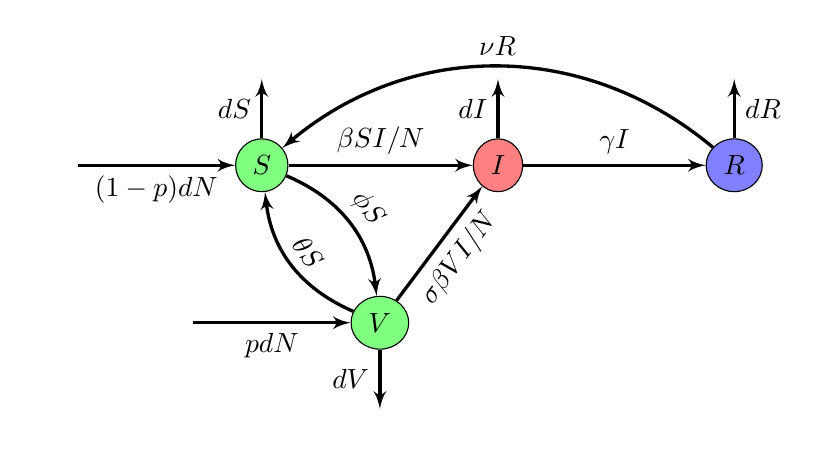
\begin{tikzpicture}[auto,
	cloud/.style={minimum width={width("N-1")+2pt},
		draw, ellipse,fill=gray!20}]
	\node [cloud, fill=green!50] at (0,0) (S) {$S$};
	\node [cloud, fill=red!50] at (3,0) (I) {$I$};
	\node [cloud, fill=blue!50] at (6,0) (R) {$R$};
	\node [cloud, fill=green!50] at (1.5, -2) (V) {$V$};
    % Births and deaths
    \node [cloud, left=2cm of S, draw=none, fill=none] (birthS) {};
    \node [cloud, left=2cm of V, draw=none, fill=none] (birthV) {};
    \node [cloud, above=0.75cm of S, draw=none, fill=none] (deathS) {};
    \node [cloud, above=0.75cm of I, draw=none, fill=none] (deathI) {};
    \node [cloud, above=0.75cm of R, draw=none, fill=none] (deathR) {};
    \node [cloud, below=0.75cm of V, draw=none, fill=none] (deathV) {};
	%% Flows
    % Births
    \path [line, very thick] (birthS) to node [midway, below, sloped] (TextNode) {$(1-p)dN$} (S);
    \path [line, very thick] (birthV) to node [midway, below, sloped] (TextNode) {$pdN$} (V);
    % Deaths
    \path [line, very thick] (S) to node [midway, left] (TextNode) {$dS$} (deathS);
    \path [line, very thick] (I) to node [midway, left] (TextNode) {$dI$} (deathI);
    \path [line, very thick] (R) to node [midway, right] (TextNode) {$dR$} (deathR);
    \path [line, very thick] (V) to node [midway, left] (TextNode) {$dV$} (deathV);
    % Regular flows
	\path [line, very thick] (S) to node [midway, above] (TextNode) {$\beta SI/N$} (I);
	\path [line, very thick] (I) to node [midway, above, sloped] (TextNode) {$\gamma I$} (R);
	\path [line, very thick, bend right=40] (R) to node [midway, above, sloped] (TextNode) {$\nu R$} (S);
    % Vaccination flows
	\path [line, very thick, bend left] (S) to node [midway, above, sloped] (TextNode) {$\phi S$} (V);
	\path [line, very thick, bend left] (V) to node [midway, above, sloped] (TextNode) {$\theta S$} (S);
	\path [line, very thick] (V) to node [midway, below, sloped] (TextNode) {$\sigma\beta VI/N$} (I);
\end{tikzpicture}
\end{document}